\documentclass{beamer}
\mode<presentation>
{
\usetheme{Berlin}
\setbeamercovered{transparent}
}

\usepackage[english]{babel}
\usepackage[latin1]{inputenc}
\usepackage{mathptmx}
\usepackage[scaled=.90]{helvet}
\usepackage{courier}
\usepackage[T1]{fontenc}

\title{Software architecture of control system for heterogeneous group of mobile
robots}

\author{Kirsanov Kirill\inst{1} dpn20605} 

\institute
{
\inst{1}
Laboratory "Sensorika", Miusskaya sq., 4, 125047, Moscow, Russia
}

\date{2014.11.28 // DAAAM International Symposium}
\begin{document}

\begin{frame}
\titlepage
\end{frame}

\begin{frame}
\frametitle{Outline}
\tableofcontents
\end{frame}

\section{Introduction}
\subsection{Robotics middleware}
\begin{frame}
\frametitle{What is robotics middleware?}
Robotics middleware is a software frameworks that provides, several
base functionalities and tools for developing and testing robotics software
modules.
It`s regulates how to express robot in computer terms (e.g. programming
language).

\vskip0pt plus.5fill

And incudes some models for:
\begin{itemize}
  \item Robotic and mechatronic devices
  \item Naming
  \item Communicating
\end{itemize}


\end{frame}


\begin{frame}
\frametitle{What is robotics middleware?}
\framesubtitle{Examples}
\begin{itemize}
\item<1> \textbf{ROS robotic Operating System}
\item<1> \textbf{Microsoft Robotics Studio} 
\item<1> \textbf{Player Project} 
\item<1> \textbf{ORCA2} 
\item<1> \textbf{LAAS/GenoM} 
\item<1> \textbf{Marie} 
\item<1> \textbf{URBI} 
\item<1> \textbf{Webots} 
\item<1> \textbf{RoboJRE}
\item<1> \textbf{OROCOS}
\item<1> \textbf{Software Development Kits for specific robots like Festo, ABB,
Kuka etc..}
\end{itemize}
\end{frame}

\subsection{Robot model in software}
\begin{frame}
\frametitle{Robot and mechatronic device model in software terms}

\begin{itemize}
\item Robots and mechatronic devices are abstracted in terms of finite state
machine (FSM)
\item Thus controlling procedure transforms into changing the states of FMS
\item This changing is implemented as messaging. Synchrous or asynchrous
\end{itemize}
This extensibility scheme for group control.

\center{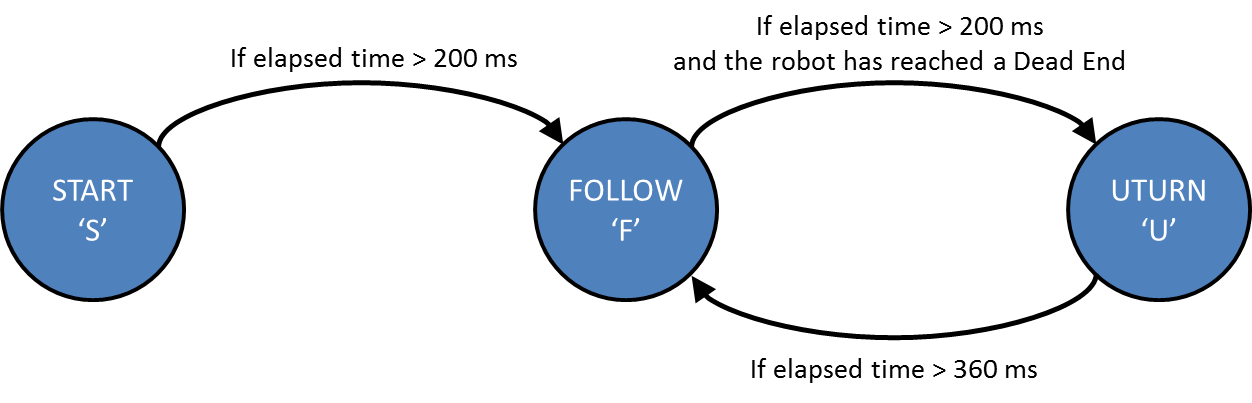
\includegraphics[width=7cm]{simplefsmdiagram.png}}

\end{frame}

\begin{frame}
\frametitle{Necessary procedures}

\begin{itemize}
\item Naming and addressing - how to find device in computer space
\item Messaging - how to read or change states of FMS
\item Aggregating - how to to assemple a robot or group of robots from 
plurality of devices
\end{itemize}


The closest analogue is the WWW: \textbf{Naming and adressing} - DNS servers and
site names like www.daaam.info, \textbf{messaging} - HTTP protocol,
\textbf{agregating} - Internet Browser, which uses a series of HTTP requests to show web page
\end{frame}
\section{Proposed architecure}

\begin{frame}
\frametitle{Proposed architecure}

\framesubtitle{Restrictions}

\begin{itemize}
  \item Multiplatfom - x86, arm, avr and Language-independed
  \item Error recovery and auto configuration
  \item Small enough that would fit onboard computer
  \item Fast prototyping
\end{itemize}

\center{
	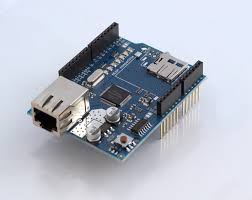
\includegraphics[width=3cm]{arduino.jpg}
	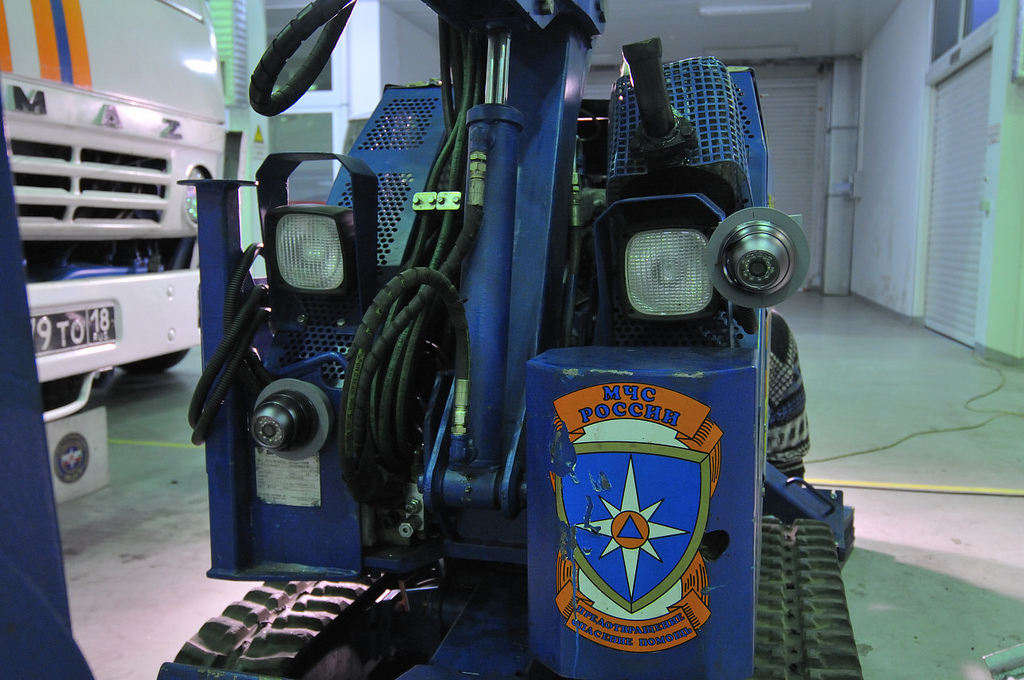
\includegraphics[width=3.5cm]{brokk.jpg}
	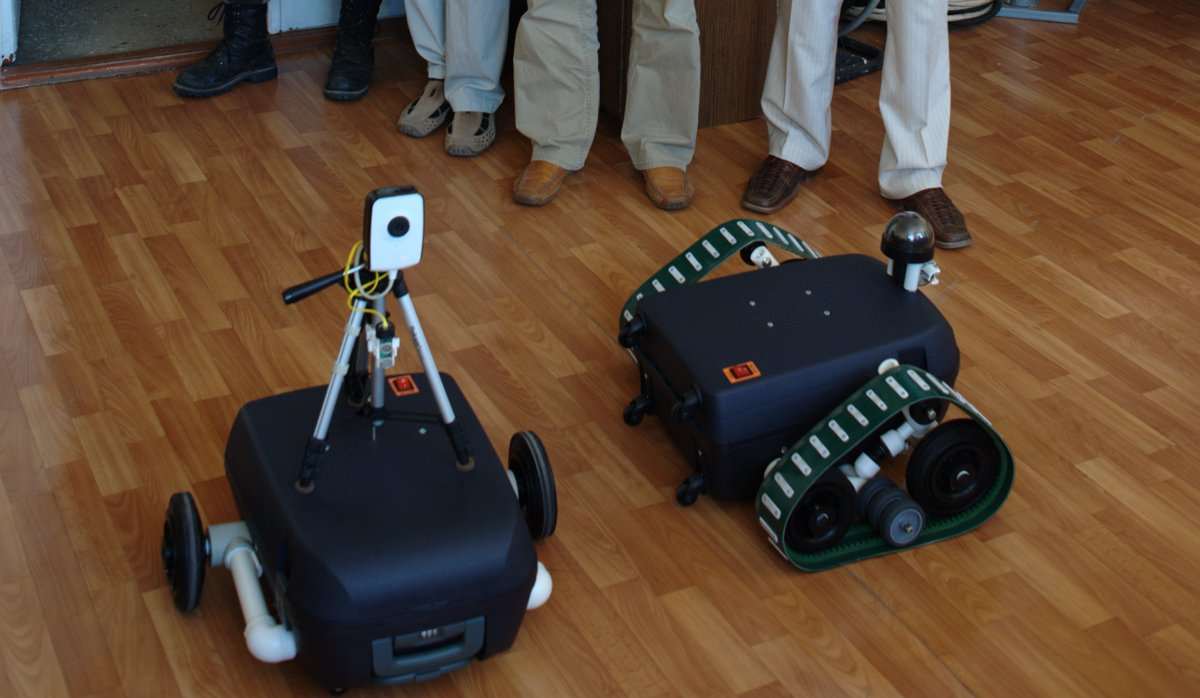
\includegraphics[width=4cm]{amur2.jpg}
		
}
\end{frame}

\subsection{Naming and addresing}
\begin{frame}
\frametitle{Naming and addresing scheme}
Whel known Tree model:
\begin{itemize}
  \item Can be flattened into into string:
  \emph{'Place->Laboratory->Robot->Device->SubDevice'} or
  \emph{'ip addres>Port'}
  \item Easy to excpress in programming languages
\end{itemize}
\center{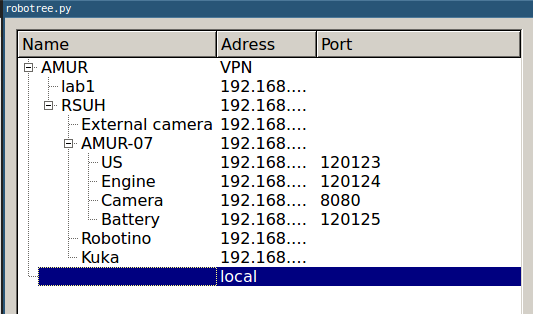
\includegraphics[width=5cm]{tree.png}}

\end{frame}

\subsection{Discovery}
\begin{frame}
\frametitle{Discovery scheme}
\begin{itemize}
\item Before you start working with something that is to be found.
In the real world, this procedure is obvious, but it is
necessary to implement appropriate search pattern in computer space. 
\item To ensure that it was implemented special service - Naming Service
\item Every Device automaticly registrating on it at statrup
\item Every NameSrver periodically scans the network for its copies and
exchanges information about devices. This protocol based on Distributed hash
table (DHT) algorithm.
\end{itemize}
\end{frame}

\begin{frame}
\framesubtitle{Discovery scheme Implementation}
\center{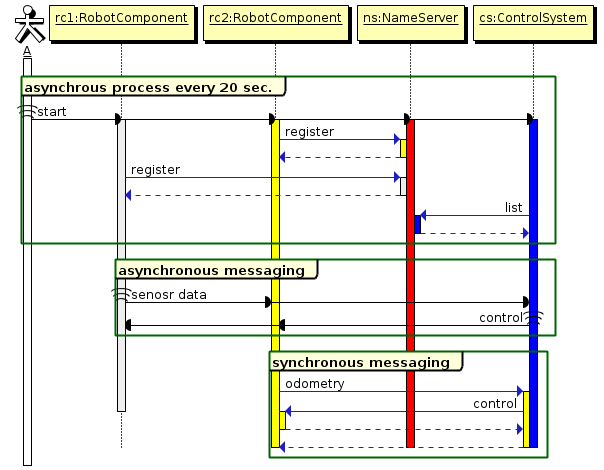
\includegraphics[width=8cm]{nameserver.png}}
\end{frame}

\subsection{Messaging}
\begin{frame}
\begin{itemize}
  \item At bottom lever 0ZMQ network library are used 
  \item At top lever messages are JSON encoded
  \item Each message contains timestamp and serial number,that allow to
  restore the sequence of messages and determine the losses in the asynchronous mode
\end{itemize}
\center{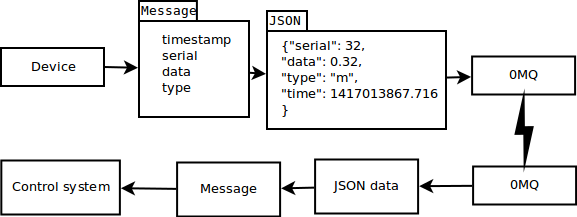
\includegraphics[width=8cm]{messaging.png}}

(Inspired by Erlang programming language)

\end{frame}

\subsubsection{Error Recovery}
\begin{frame}
\frametitle{Error recovery and updating software at runtime}
\begin{itemize}
  \item When the device is disconnected there is no disconnection on the
  upper (messaging) level
  \item When the device is back - there is no need to re-establish connection
  manually
  \item All messages are stored in Nameservers, so that it becomes possible to
  obtain old data or forgone due to errors or software update
\end{itemize}
\center{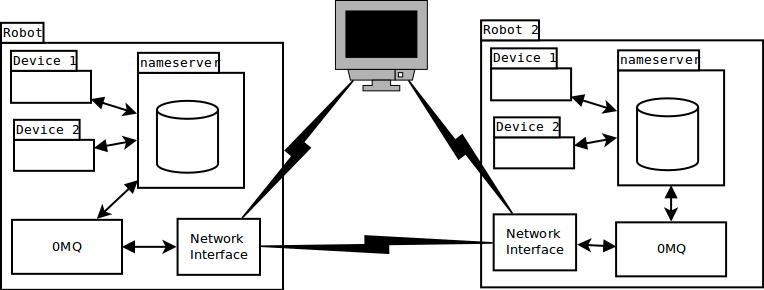
\includegraphics[width=7cm]{messaging2.png}}

\end{frame}


\subsubsection{Type interface}
\begin{frame}
\frametitle{Type interface}
\framesubtitle{}
\begin{itemize}
  \item To specify message type the SI (International System of Units) are used over
traditional programming language datetypes
\item For example in conventional systems the distance, speed and temperature
are stored using \emph{double} datatype. This may lead to unexpected errors and
makes it difficult to document
\item Implementation of SI as a type system of programming language provide more
robustness and ease of domentating.
\item Hindley-Milner (HM) algorithm are used to check types.
\end{itemize}
\end{frame}

\section{Conclusion}

\subsection{Test Results}
\begin{frame}
Dependence of time of the transmission on the data size over WiFi.
\center{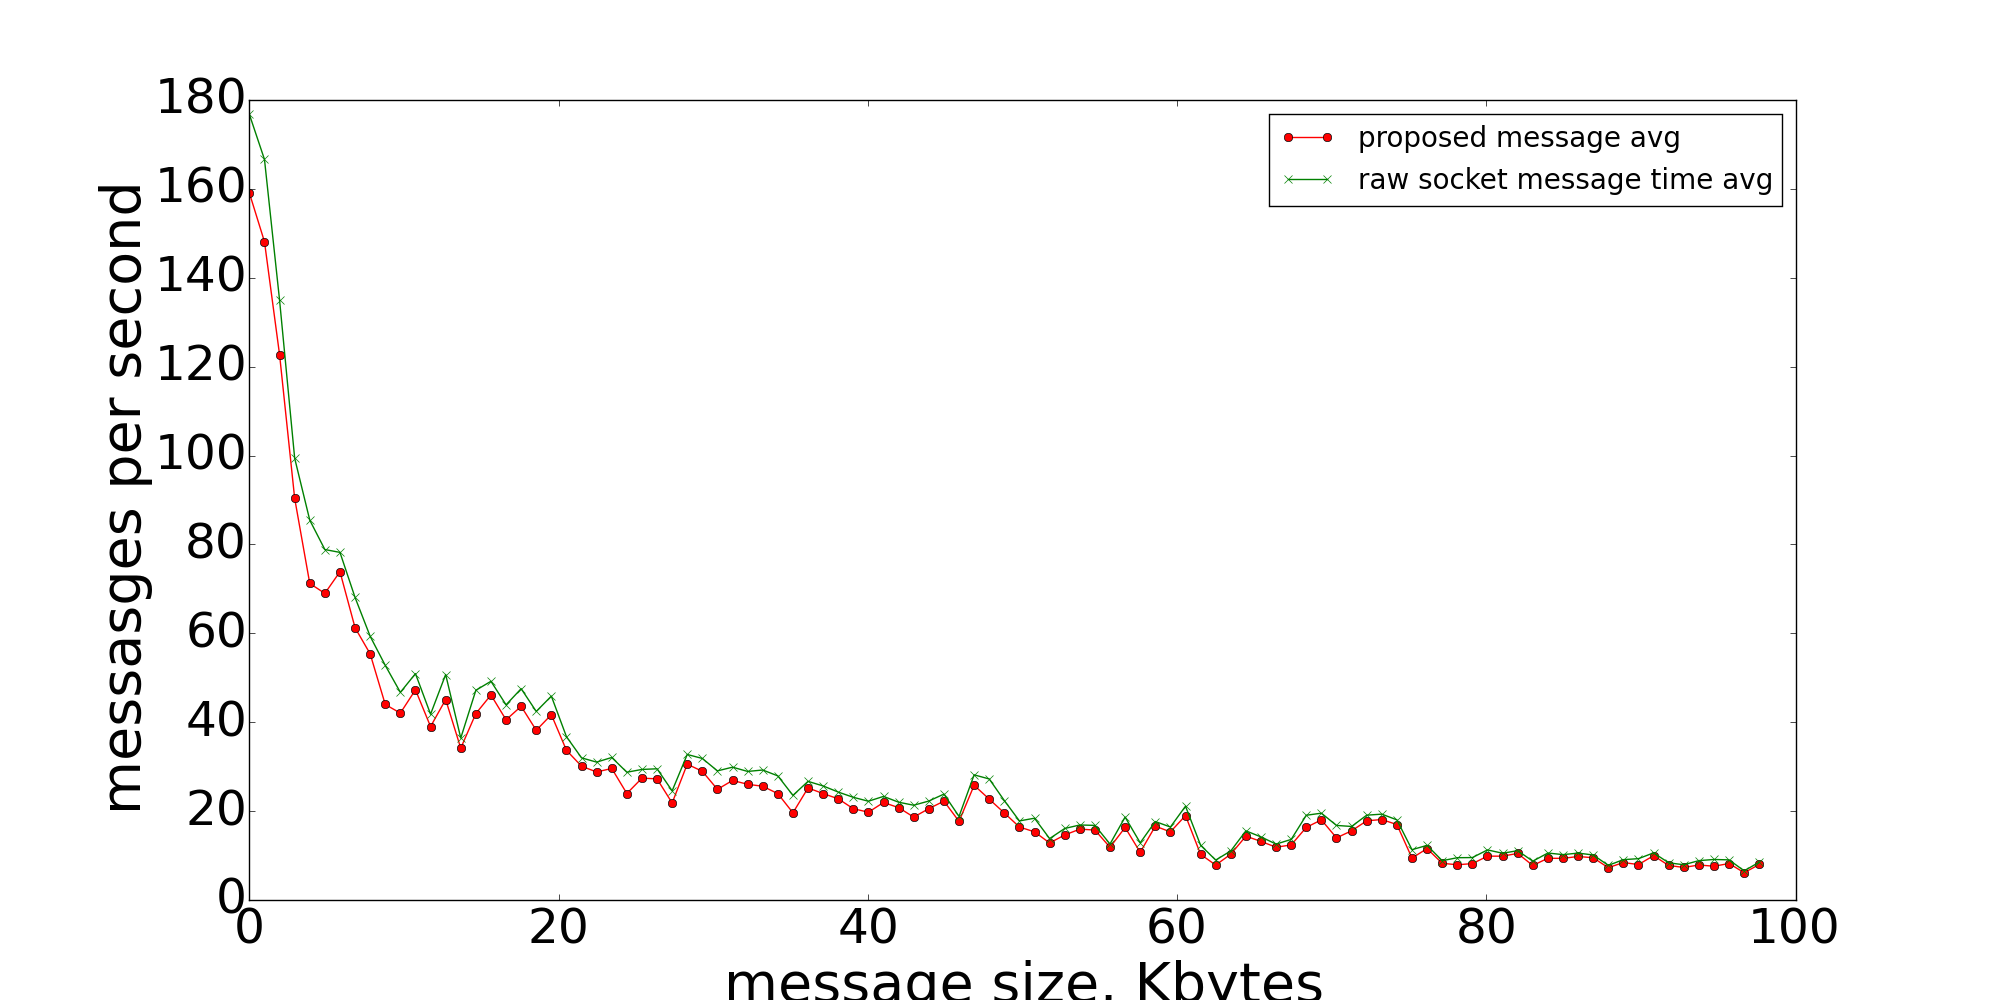
\includegraphics[width=11cm]{ping2.png}} \\
100 sequential synchronous messages(200 total) are used for each step. On each
step data are randomized

\end{frame}
\subsection{Summary}
\begin{frame}

\frametitle{Summary}
\begin{itemize}
  \item New message-orientated software architecture are proposed
  \item DHT algorithm supports the integrity of control system by replicating
  metadata
  \item Network error-tolerance are provided by messaging model (actor-model)
  \item Using International System of Units for type annotations and
  Hindley-Milner algorithm for type-checking provides a limited ability to
  detect typing errors
\end{itemize}
\end{frame}

%\subsection{Future work}


%\begin{frame}
%\frametitle{}
%\framesubtitle{}

%\end{frame}

\end{document}
